% !TEX root = ../main.tex

\subsection{Results}
With the implementation and analysis out of the way, we can begin to experiment with the echo effect. We have one parameter to adjust: The delay \emph{d}. We have taken a binary approach, starting from Fs and halving the delay each time. The results are shown in \cref{tbl:echo}.
\begin{table}[!hbt]
	\centering
	\begin{tabular}{ccc}
		\toprule
		Units of delay & Time [ms] & Effect \\ 
		\midrule
		44100 & 1000 & Late echo \\ 
		22050 & 500 & Late echo \\ 
		11025 & 250 & Echo \\ 
		5513 & 125 & Echo \\ 
		2757 & 62.5 & Hard to distinguish tracks \\ 
		1379 & 31.3 & Hard to distinguish tracks \\ 
		690 & 15.6 & Impossible to distinguish tracks \\ 
		173 & 3.9 & Impossible to distinguish tracks \\ 
		\bottomrule
	\end{tabular}
	\caption{Effect of different delays for the echo effect, sample rate of \SI{44100}{\hertz}. Sample used is \cite{audiohello}.}
	\label{tbl:echo}
\end{table}
For the last samples, not only is it impossible to distinguish the tracks, the perceived pitch of the vocal track is also changed. For the cases where the delay is around \SI{50}{\milli\second}, we get the effect we wish to dive in to later: Chorus.

For delays larger than around \SI{100}{\milli\second} we get the effect we are looking for. If we increase the delay even further, the echo effect gets more pronounced. For short samples like the vocal hello track used here, the delay gets large enough to completely separate the two tracks. A visualization of the effects for the longer delays is shown in \cref{fig:echohello}. \fxnote{Insert comment on monkey island here}

\begin{figure}[!hbt]
	\centering
	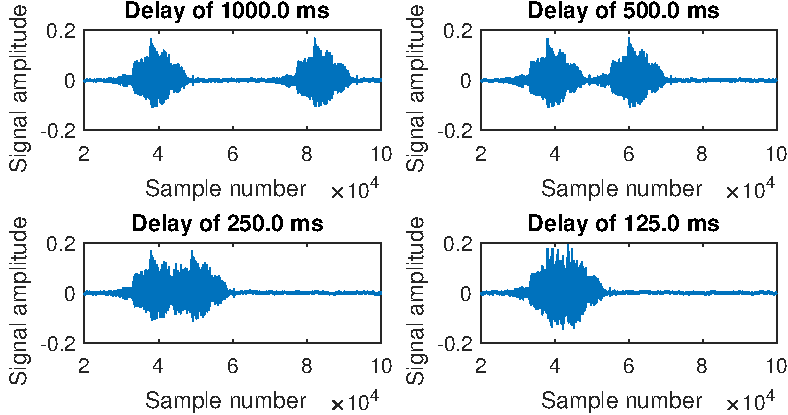
\includegraphics[width=\textwidth]{EchoHello.pdf}
	\caption{Visualization of the echo effect on a track. Sample is from \cite{audiohello}. It can clearly be seen, how the echo joins the main track in time, as the echo delay is reduced.}
	\label{fig:echohello}
\end{figure}
